\documentclass[]{beamer}\usepackage[]{graphicx}\usepackage[]{color}
% maxwidth is the original width if it is less than linewidth
% otherwise use linewidth (to make sure the graphics do not exceed the margin)
\makeatletter
\def\maxwidth{ %
  \ifdim\Gin@nat@width>\linewidth
    \linewidth
  \else
    \Gin@nat@width
  \fi
}
\makeatother

\definecolor{fgcolor}{rgb}{0.345, 0.345, 0.345}
\newcommand{\hlnum}[1]{\textcolor[rgb]{0.686,0.059,0.569}{#1}}%
\newcommand{\hlstr}[1]{\textcolor[rgb]{0.192,0.494,0.8}{#1}}%
\newcommand{\hlcom}[1]{\textcolor[rgb]{0.678,0.584,0.686}{\textit{#1}}}%
\newcommand{\hlopt}[1]{\textcolor[rgb]{0,0,0}{#1}}%
\newcommand{\hlstd}[1]{\textcolor[rgb]{0.345,0.345,0.345}{#1}}%
\newcommand{\hlkwa}[1]{\textcolor[rgb]{0.161,0.373,0.58}{\textbf{#1}}}%
\newcommand{\hlkwb}[1]{\textcolor[rgb]{0.69,0.353,0.396}{#1}}%
\newcommand{\hlkwc}[1]{\textcolor[rgb]{0.333,0.667,0.333}{#1}}%
\newcommand{\hlkwd}[1]{\textcolor[rgb]{0.737,0.353,0.396}{\textbf{#1}}}%
\let\hlipl\hlkwb

\usepackage{framed}
\makeatletter
\newenvironment{kframe}{%
 \def\at@end@of@kframe{}%
 \ifinner\ifhmode%
  \def\at@end@of@kframe{\end{minipage}}%
  \begin{minipage}{\columnwidth}%
 \fi\fi%
 \def\FrameCommand##1{\hskip\@totalleftmargin \hskip-\fboxsep
 \colorbox{shadecolor}{##1}\hskip-\fboxsep
     % There is no \\@totalrightmargin, so:
     \hskip-\linewidth \hskip-\@totalleftmargin \hskip\columnwidth}%
 \MakeFramed {\advance\hsize-\width
   \@totalleftmargin\z@ \linewidth\hsize
   \@setminipage}}%
 {\par\unskip\endMakeFramed%
 \at@end@of@kframe}
\makeatother

\definecolor{shadecolor}{rgb}{.97, .97, .97}
\definecolor{messagecolor}{rgb}{0, 0, 0}
\definecolor{warningcolor}{rgb}{1, 0, 1}
\definecolor{errorcolor}{rgb}{1, 0, 0}
\newenvironment{knitrout}{}{} % an empty environment to be redefined in TeX

\usepackage{alltt}
%\documentclass[handout]{beamer}
%\usepackage[dvips]{color}
\usepackage{graphicx}
\usepackage{amsmath,amssymb,array,eucal}
\usepackage{xcolor}
\definecolor{beamer@blendedblue}{RGB}{86,155,189}
\definecolor{myblue}{RGB}{12,76,138}
\setbeamercolor{structure}{fg=myblue}
\definecolor{Ftitle}{RGB}{12,76,138}
\definecolor{Descitem}{RGB}{238,238,244}
\definecolor{StdTitle}{RGB}{12,76,138}
\definecolor{StdBody}{RGB}{213,24,0}
\definecolor{StdBody}{RGB}{213,24,0}

\definecolor{AlTitle}{RGB}{255, 190, 190}
\definecolor{AlBody}{RGB}{213,24,0}

\definecolor{ExTitle}{RGB}{201, 217, 217}
\definecolor{ExBody}{RGB}{213,24,0}

\setbeamercolor{frametitle}{fg = Ftitle}
\setbeamercolor{title}{fg = Ftitle}
\setbeamercolor{item}{fg = Ftitle}
\setbeamercolor{subitem}{fg = Ftitle}
\setbeamercolor{subsubitem}{fg = Ftitle}
\setbeamercolor{description item}{fg = myblue}
\setbeamercolor{titlelike}{fg=myblue}

\DeclareMathOperator{\sgn}{sgn}
\newcommand{\e}{\mathbf{e}}
\renewcommand{\P}{\mathbf{P}}
\newcommand{\F}{\mathbf{F}}
\newcommand{\R}{\textsf{R}}
\newcommand{\mat}[1] {\mathbf{#1}}
%\newcommand{\ind}{\mathrel{\mathop{\sim}\limits^{\mathit{ind}}}}
%\newcommand{\iid}{\mathrel{\mathop{\sim}\limits^{\mathit{iid}}}}
\newcommand{\E}{\textsf{E}}
\newcommand{\SE}{\textsf{SE}}
\newcommand{\SSE}{\textsf{SSE}}
\newcommand{\RSS}{\textsf{RSS}}
\newcommand{\FSS}{\textsf{FSS}}
\renewcommand{\SS}{\textsf{SS}}
\newcommand{\MSE}{\textsf{MSE}}
\newcommand{\SSR}{\textsf{SSR}}
\newcommand{\Be}{\textsf{Beta}}
\newcommand{\St}{\textsf{St}}
\newcommand{\Ca}{\textsf{C}}
\newcommand{\Exp}{\textsf{Exp}}
\newcommand{\GDP}{\textsf{GDP}}
\newcommand{\NcSt}{\textsf{NcSt}}
\newcommand{\Bin}{\textsf{Bin}}
\newcommand{\NB}{\textsf{NegBin}}
\renewcommand{\NG}{\textsf{NG}}
\newcommand{\N}{\textsf{N}}
\newcommand{\Ber}{\textsf{Ber}}
\newcommand{\Poi}{\text{Poi}}
\newcommand{\Gam}{\textsf{Gamma}}
\newcommand{\BB}{\textsf{BB}}
\newcommand{\Gm}{\textsf{G}}
\newcommand{\Un}{\textsf{Unif}}
\newcommand{\Ex}{\textsf{Exp}}
\newcommand{\DE}{\textsf{DE}}
\newcommand{\tr}{\textsf{tr}}
\newcommand{\cF}{{\cal{F}}}
\newcommand{\cL}{{\cal{L}}}
\newcommand{\cI}{{\cal{I}}}
\newcommand{\cB}{{\cal{B}}}
\newcommand{\cP}{{\cal{P}}}
\newcommand{\bbR}{\mathbb{R}}
\newcommand{\bbN}{\mathbb{N}}
\newcommand{\pperp}{\mathrel{{\rlap{$\,\perp$}\perp\,\,}}}
\newcommand{\OFP}{(\Omega,\cF, \P)}
\newcommand{\eps}{\boldsymbol{\epsilon}}
\newcommand{\1}{\mathbf{1}_n}
\newcommand{\gap}{\vspace{8mm}}
\newcommand{\ind}{\mathrel{\mathop{\sim}\limits^{\rm ind}}}
\newcommand{\simiid}{\ensuremath{\mathrel{\mathop{\sim}\limits^{\rm
iid}}}}
\newcommand{\eqindis}{\ensuremath{\mathrel{\mathop{=}\limits^{\rm D}}}}
\newcommand{\iid}{\textit{i.i.d.}}
\newcommand{\SSZ}{S_{zz}}
\newcommand{\SZW}{S_{zw}}
\newcommand{\Var}{\textsf{Var}}
\newcommand{\corr}{\textsf{corr}}
\newcommand{\diag}{\textsf{diag}}
\newcommand{\var}{\textsf{var}}
\newcommand{\Cov}{\textsf{Cov}}
\newcommand{\Sam}{{\cal S}}
\def\H{\mathbf{H}}
\newcommand{\I}{\mathbf{I}}
\newcommand{\Y}{\mathbf{Y}}
\newcommand{\tY}{\tilde{\mathbf{Y}}}
\newcommand{\Yhat}{\hat{\mathbf{Y}}}
\newcommand{\Yobs}{\mathbf{Y}_{{\cal S}}}
\newcommand{\barYobs}{\bar{Y}_{{\cal S}}}
\newcommand{\barYmiss}{\bar{Y}_{{\cal S}^c}}
\def\bv{\mathbf{b}}
\def\X{\mathbf{X}}
\def\tX{\tilde{\mathbf{X}}}
\def\x{\mathbf{x}}
\def\xbar{\bar{\mathbf{x}}}
\def\Xbar{\bar{\mathbf{X}}}
\def\Xg{\mathbf{X}_{\boldsymbol{\gamma}}}
\def\Ybar{\bar{\Y}}
\def\ybar{\bar{y}}
\def\y{\mathbf{y}}
\def\Yf{\mathbf{Y_f}}
\def\W{\mathbf{W}}
\def\L{\mathbf{L}}
\def\w{\mathbf{w}}
\def\U{\mathbf{U}}
\def\V{\mathbf{V}}
\def\Q{\mathbf{Q}}
\def\Z{\mathbf{Z}}
\def\z{\mathbf{z}}
\def\v{\mathbf{v}}
\def\u{\mathbf{u}}

\def\zero{\mathbf{0}}
\def\one{\mathbf{1}}
\newcommand{\taub}{\boldsymbol{\tau}}
\newcommand{\betav}{\boldsymbol{\beta}}
\newcommand{\alphav}{\boldsymbol{\alpha}}
\newcommand{\A}{\mathbf{A}}
\def\a{\mathbf{a}}
\def\K{\mathbf{K}}
\newcommand{\B}{\mathbf{B}}
\def\b{\boldsymbol{\beta}}
\def\bhat{\hat{\boldsymbol{\beta}}}
\def\btilde{\tilde{\boldsymbol{\beta}}}
\def\tb{\boldsymbol{\theta}}
\def\bg{\boldsymbol{\beta_\gamma}}
\def\bgnot{\boldsymbol{\beta_{(-\gamma)}}}
\def\mub{\boldsymbol{\mu}}
\def\tmub{\tilde{\boldsymbol{\mu}}}
\def\muhat{\hat{\boldsymbol{\mu}}}
\def\tb{\boldsymbol{\theta}}
\def\tk{\boldsymbol{\theta}_k}
\def\tj{\boldsymbol{\theta}_j}
\def\Mk{\boldsymbol{{\cal M}}_k}
\def\M{\boldsymbol{{\cal M}}}
\def\Mj{\boldsymbol{{\cal M}}_j}
\def\Mi{\boldsymbol{{\cal M}}_i}
\def\Mg{{\boldsymbol{{\cal M}_\gamma}}}
\def\Mnull{\boldsymbol{{\cal M}}_{N}}
\def\gMPM{\boldsymbol{\gamma}_{\text{MPM}}}
\def\gHPM{\boldsymbol{\gamma}_{\text{HPM}}}
\def\Mfull{\boldsymbol{{\cal M}}_{F}}
\def\tg{\boldsymbol{\theta}_{\boldsymbol{\gamma}}}
\def\g{\boldsymbol{\gamma}}
\def\eg{\boldsymbol{\eta}_{\boldsymbol{\gamma}}}
\def\G{\mathbf{G}}
\def\cM{\cal M}
\def\D{\Delta}
\def \shat{{\hat{\sigma}}^2}
\def\uv{\mathbf{u}}
\def\l {\lambda}
\def\d{\delta}
\def\Sigmab{\boldsymbol{\Sigma}}
\def\Lambdab{\boldsymbol{\Lambda}}
\def\lambdab{\boldsymbol{\lambda}}
\def\Mg{{\cal M}_\gamma}
\def\S{{\cal{S}}}
\def\qg{p_{\boldsymbol{\gamma}}}
\def\pg{p_{\boldsymbol{\gamma}}}
%\def\t{\mathbf{t}}
\def\T{\boldsymbol{\Theta}}
\def\Tb{\boldsymbol{\Theta}}
\def\t{\mathbf{t}}

\usepackage{verbatim}

\usetheme{default}
\title{G-Priors and Mixture Distributions}
\institute{Merlise Clyde}
\author{STA721 Linear Models Duke University}
\date{\today}
%\logo{duke.eps}
\IfFileExists{upquote.sty}{\usepackage{upquote}}{}
\begin{document}


\maketitle

\begin{frame}
  \frametitle{Bayesian Estimation}
  Model
$$
\Y \sim \N(\X \b, \I_n/\phi)
$$
with precision $\phi = 1/\sigma^2$.
\pause

\vfill
Default Prior Choices for $\b$ and $\phi$:
\begin{itemize}
\item ``Non-Informative Priors'': Independent Jeffreys' Priors (improper)
\item g-prior  $\N(0, \frac{g}{\phi}(\X^T\X)^{-1})$
\item Partitioned g-priors
\item Zellner-Siow Cauchy Prior, mixtures and MCMC (if time)
\end{itemize}

Readings: Hoff Chapter 9
\end{frame}



\begin{frame}
  \frametitle{Zellner's $g$-prior}
Zellner's g-prior(s) $\b \mid \phi \sim \N(\bv_0, g
    (\X^T\X)^{-1}/\phi)$ \pause

$$\b \mid \Y, \phi \sim \N\left( \frac{g}{1 + g} \bhat +  \frac{1}{1 + g}
\bv_0, \frac{g}{1 + g} (\X^T\X)^{-1} \phi^{-1} \right)$$ \pause



\vspace{1in}
 Invariance: Require posterior of   $\X \b$  equal the posterior of $\X \H \alphav$
\pause   ($\a_0 = \H^{-1} \bv_0$)



\end{frame}

\begin{frame}
  \frametitle{Shrinkage}
 Posterior mean under  $g$-prior  with $\bv_0 = 0$
$\frac{g}{1 +g} \bhat $

\centerline{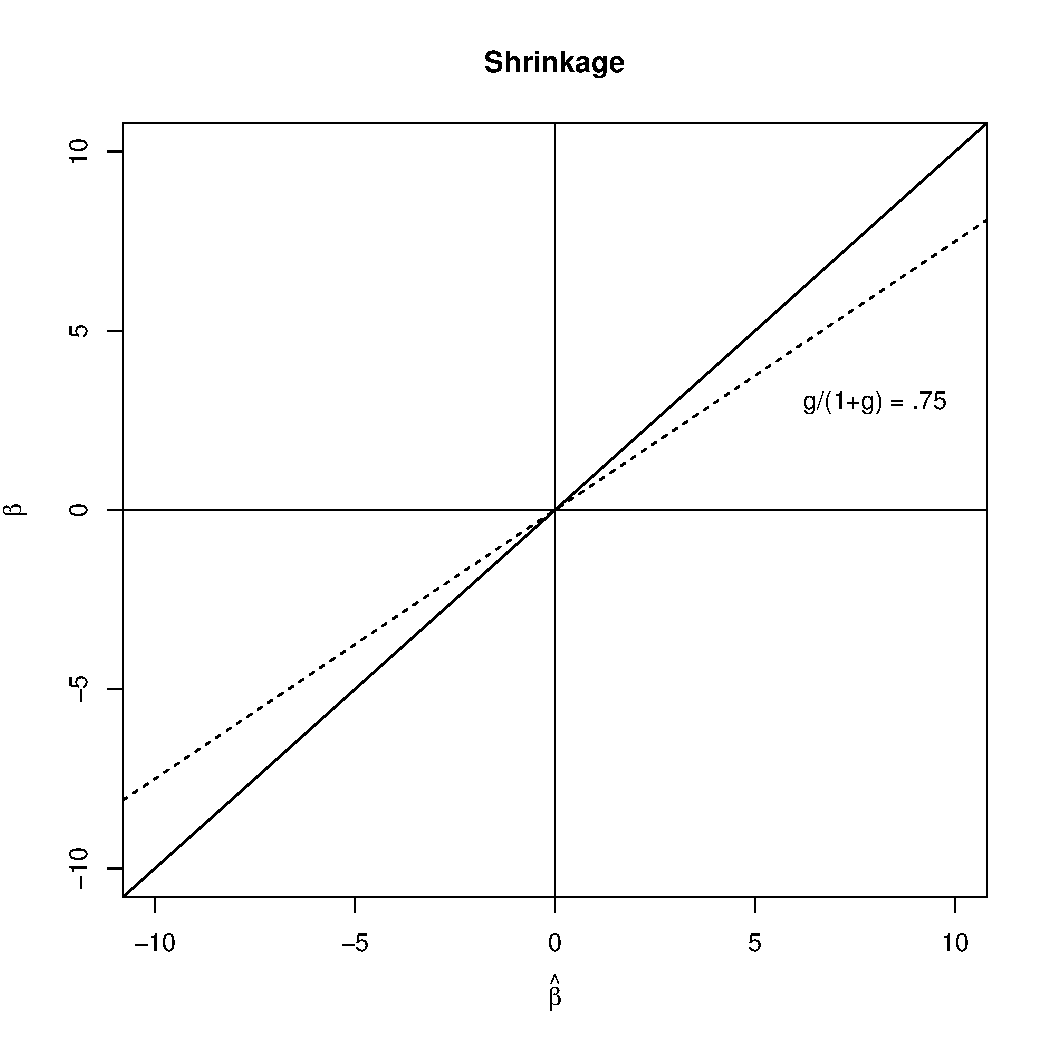
\includegraphics[height=3in]{shrinkage}}
\end{frame}


\begin{frame} \frametitle{Choice of $g$}
\begin{itemize}
  \item $\frac{g}{1 + g}$  weight given to the data \pause
  \item Fixed $g$ effect does not vanish as $n \to \infty$  (asymptotic bias) \pause
  \item Use $g = n$ or place a prior distribution on $g$
\end{itemize}
\end{frame}


\begin{frame}
 \frametitle{Partitioned Zellner's $g$-prior }

Zellner recognized that some parameters might have less information

$$ \Y = \X_0 \b_0 + \X_1 \b_1 + \eps$$

\begin{itemize}
\item $\X_0^T \X_1 = \zero$ (orthogonal columns) \pause
\item Fisher information block diagonal \pause
\item $\b_0 \sim N( \bv_0,  g_0 (\X_0^T\X_0)^{-1}/\phi)$ \pause
\item $\b_1 \sim N( \bv_1,  g_1 (\X_1^T\X_1)^{-1}/\phi)$ \pause
\item $p(\phi) \propto 1/\phi$
\end{itemize}
Special case $\X_0 = \one_n$ and let $g_0 \to \infty$
$$p(\beta_0, \phi) \propto 1/\phi$$
\end{frame}

\begin{frame}[t]
  \frametitle{Bayesian Estimation with $g$ prior}

\begin{eqnarray*}
\Y & = & \one \alpha_0 + \X_1 \b + \eps \\
p(\alpha_0, \phi) & \propto & 1 \\
\b \mid \phi & \sim & \N(\zero, \frac{g}{\phi} (\X^T (\I_n - \P_{\one}) \X)^{-1})
\end{eqnarray*}\pause

Equivalent to
\begin{eqnarray*}
\Y & = & \one \beta_0 + \I_n - \P_1) \X_1 \b + \eps \\
\beta_0 & = & \alpha + \bar{\x}^T \b \\
p(\beta_0, \phi) & \propto & 1 \\
\b \mid \phi & \sim & \N(\zero, \frac{g}{\phi} (\X^T (\I_n - \P_{\one}) \X)^{-1})
\end{eqnarray*}
\end{frame}

\begin{frame}\frametitle{Prior Data}
Note $$(\X^T (\I_n - \P_{\one}) \X) = (\X^T (\I_n - \P_{\one})^T (\I_n
- \P_{\one}) \X)  = (\X -\one_n \Xbar^T)^T (\X - \one_n \Xbar) $$
\pause
Let  $(\X -\one_n \Xbar^T)^T (\X - \one \Xbar) = \SS_{\X} = \U^T \U$
\pause

Quadratic contribution to the log likelihood from prior after integrating out $\beta_0$

$$ ( \Y_c  - \X_c \b)^T(\Y_c - \X_c\b) + ( \b^T\frac{\U^T \U}{g} \b)   $$
\pause
$$ ( \Y_c  - \X_c \b)^T(\Y_c - \X_c\b) + ( \zero_p -
\frac{\U}{\sqrt{g}}\b)^T(\zero_p -  \frac{\U}{\sqrt{g}} \b)   $$

Prior observations  with $Yc =  0$.
\end{frame}


\begin{frame}\frametitle{Example: g=5, n=30}

In SLR it is like an extra $Y_0 = 0$ at $\X_o = \sqrt{\frac{\SS_x}{g}}$:
$$ ( \Y_c  - \X_c \b)^T(\Y_c - \X_c\b) + (0 - \sqrt{\frac{\SS_x}{g}}\b)^T (0 - \sqrt{\frac{\SS_X}{g}} \b)   $$
\pause
\begin{knitrout}
\definecolor{shadecolor}{rgb}{0.969, 0.969, 0.969}\color{fgcolor}
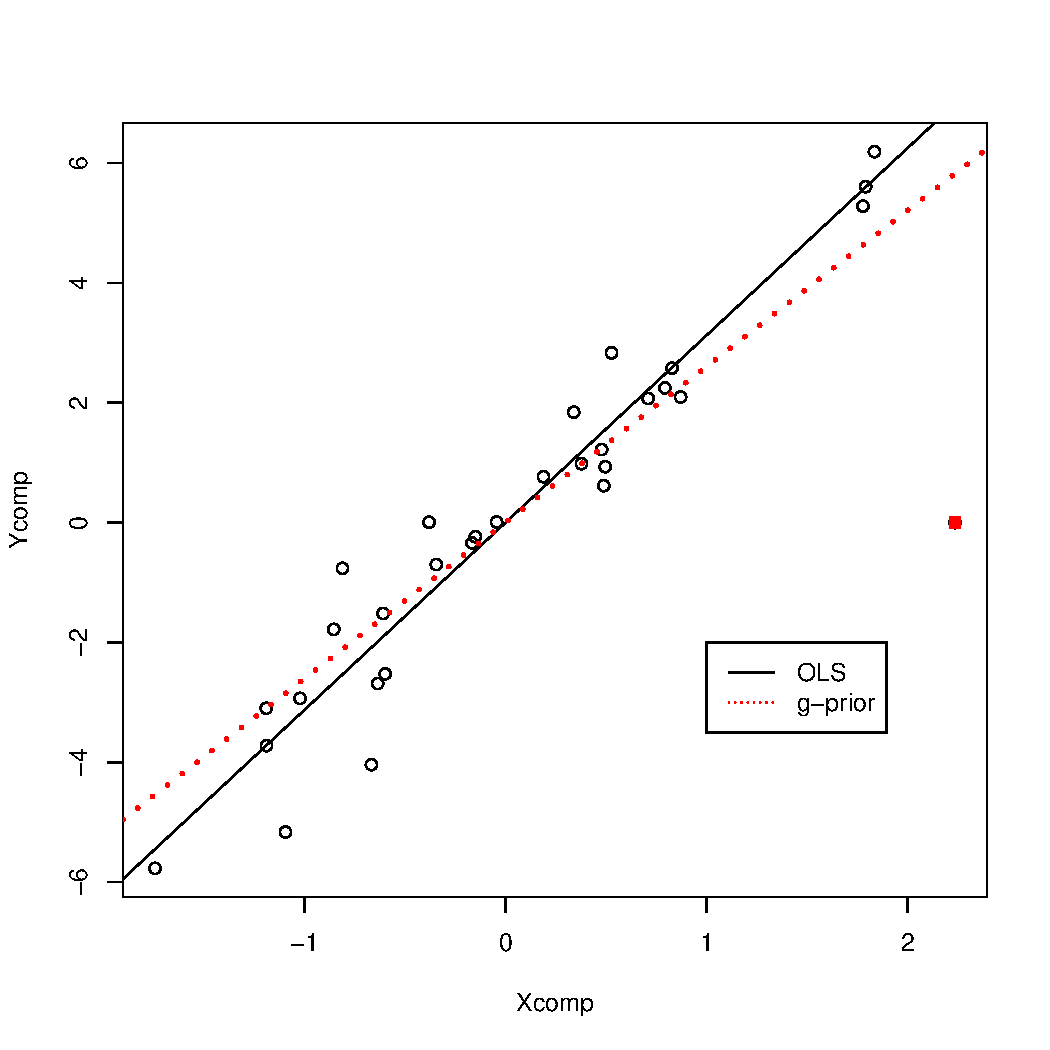
\includegraphics[width=3.5in,height=2.5in]{figure/simdata-1} 

\end{knitrout}


\end{frame}



\begin{frame}
  \frametitle{Disadvantages of Conjugate Priors}
  Disadvantages: \pause
\begin{itemize}
\item Results  may have be sensitive to prior ``outliers'' due to
  linear updating \pause
\item Problem potentially with all Normal priors, not just the
  $g$-prior. \pause
\item Cannot capture all possible prior beliefs \pause
\item Mixtures of Conjugate Priors
\end{itemize}
\end{frame}

\begin{frame}
  \frametitle{Mixtures of Conjugate Priors}
  \begin{theorem}[Diaconis \& Ylivisaker 1985]  Given a sampling model
  $p(y \mid \tb)$ from an exponential family, any prior distribution
  can be expressed as a mixture of conjugate prior distributions
 \end{theorem}

 \begin{itemize}
 \item Prior $p(\tb) = \int p(\tb \mid \omega) p(\omega)\, d \omega$ \pause
 \item Posterior \pause
   \begin{eqnarray*}
   p(\tb \mid \Y)  &\propto & \int p(\Y \mid \tb) p(\tb\mid \omega)
   p(\omega) \, d\omega \pause \\
 & \propto & \int  \frac{  p(\Y \mid \tb) p(\tb \mid \omega) } {p(\Y \mid
   \omega)}  p(\Y \mid
 \omega) p(\omega ) \, d \omega  \pause \\
& \propto & \int p(\tb \mid \Y, \omega)  p(\Y \mid
 \omega) p(\omega ) \, d \omega \pause \\
 p(\tb \mid \Y) & =  & \frac{\int p(\tb \mid \Y, \omega)  p(\Y \mid
 \omega) p(\omega ) \, d \omega }
{\int p(\Y \mid
 \omega) p(\omega ) \, d \omega }
       \end{eqnarray*}

 \end{itemize}
\end{frame}

\begin{frame}
  \frametitle{Zellner-Siow prior (assume $\X$ is centered)}
Zellner's g-prior $\b \mid \phi \sim \N(\zero_p, g
    (\X^T\X)^{-1}/\phi)$ \pause

\begin{itemize}
\item Choice of $g$?  \pause
\item $\frac{g}{1 + g}$  weight given to the data \pause
\item Let $\tau = 1/g$ assign $\tau \sim G(1/2, n/2)$ \pause
\item Marginal prior on $\b \sim C(0, \phi^{-1} \X^T\X)$
\item Can express posterior as a mixture of $g$-priors
$$p(\tau \mid \Y) = \frac{p(\Y \mid \tau) p(\tau)}{\int p(\Y \mid \tau) p(\tau) \, d \tau}$$ \pause
\item Problem:  no analytic expression for integral \pause
\item Need 2 one dimensional integrals to obtain posterior. \pause
\item What about credible intervals?
\end{itemize}
\end{frame}

\begin{frame}[t] \frametitle{Markov Chain Monte Carlo}
\begin{itemize}
\item We know that $\beta_0, \b, \phi \mid \Y, g=1/\tau$ has a Normal-Gamma distribution  \pause
\item We can show that $\tau \mid \beta_0,\b, \phi, \Y$ has a Gamma distribution \pause
$$p(\tau \mid \b, \phi, \Y) \propto {\cal{L}}(\beta_0,\b, \phi)
\tau^{p/2} e^{( - \tau \frac{\phi}{2} \b^T (\X^T\X) \b)}
\tau^{1/2 - 1} e^{ - \tau n/2}$$ \pause
\item alternate sampling from full conditional distributions given current values of other parameters.  (STA 601) \pause
\item JAGS or STAN
\end{itemize}
\end{frame}


\begin{frame}[fragile]{JAGS Code: library(R2jags)}
\begin{knitrout}
\definecolor{shadecolor}{rgb}{0.969, 0.969, 0.969}\color{fgcolor}\begin{kframe}
\begin{alltt}
\hlstd{model} \hlkwb{=} \hlkwa{function}\hlstd{()\{}
  \hlkwa{for} \hlstd{(i} \hlkwa{in} \hlnum{1}\hlopt{:}\hlstd{n) \{}
      \hlstd{Y[i]} \hlopt{~} \hlkwd{dnorm}\hlstd{(beta0}\hlopt{+} \hlstd{(X[i]} \hlopt{-}\hlstd{Xbar)}\hlopt{*}\hlstd{beta, phi)}
  \hlstd{\}}
  \hlstd{beta0} \hlopt{~} \hlkwd{dnorm}\hlstd{(}\hlnum{0}\hlstd{,} \hlnum{.000001}\hlopt{*}\hlstd{phi)} \hlcom{#precision is 2nd arg}
  \hlstd{beta} \hlopt{~} \hlkwd{dnorm}\hlstd{(}\hlnum{0}\hlstd{, phi}\hlopt{*}\hlstd{tau}\hlopt{*}\hlstd{SSX)}  \hlcom{#precision is 2nd arg}
  \hlstd{phi} \hlopt{~} \hlkwd{dgamma}\hlstd{(}\hlnum{.001}\hlstd{,} \hlnum{.001}\hlstd{)}
  \hlstd{tau} \hlopt{~} \hlkwd{dgamma}\hlstd{(}\hlnum{.5}\hlstd{,} \hlnum{.5}\hlopt{*}\hlstd{n)}
  \hlstd{g} \hlkwb{<-} \hlnum{1}\hlopt{/}\hlstd{tau}
  \hlstd{sigma} \hlkwb{<-} \hlkwd{pow}\hlstd{(phi,} \hlopt{-}\hlnum{.5}\hlstd{)}
\hlstd{\}}
\hlstd{data} \hlkwb{=} \hlkwd{list}\hlstd{(}\hlkwc{Y}\hlstd{=Y,} \hlkwc{X}\hlstd{=X,} \hlkwc{n} \hlstd{=}\hlkwd{length}\hlstd{(Y),} \hlkwc{SSX}\hlstd{=}\hlkwd{sum}\hlstd{(Xc}\hlopt{^}\hlnum{2}\hlstd{),}
            \hlkwc{Xbar}\hlstd{=}\hlkwd{mean}\hlstd{(X))}
\hlstd{ZSout} \hlkwb{=} \hlkwd{jags}\hlstd{(data,} \hlkwc{inits}\hlstd{=}\hlkwa{NULL}\hlstd{,}
             \hlkwc{parameters.to.save}\hlstd{=}\hlkwd{c}\hlstd{(}\hlstr{"beta0"}\hlstd{,}\hlstr{"beta"}\hlstd{,} \hlstr{"g"}\hlstd{,}
                                  \hlstr{"sigma"}\hlstd{),}
             \hlkwc{model}\hlstd{=model,} \hlkwc{n.iter}\hlstd{=}\hlnum{10000}\hlstd{)}
\end{alltt}


{\ttfamily\noindent\itshape\color{messagecolor}{\#\# module glm loaded}}\begin{verbatim}
## Compiling model graph
##    Resolving undeclared variables
##    Allocating nodes
## Graph information:
##    Observed stochastic nodes: 30
##    Unobserved stochastic nodes: 4
##    Total graph size: 174
## 
## Initializing model
\end{verbatim}
\end{kframe}
\end{knitrout}
\end{frame}

\begin{frame}[fragile] \frametitle{HPD intervals}



\begin{knitrout}
\definecolor{shadecolor}{rgb}{0.969, 0.969, 0.969}\color{fgcolor}\begin{kframe}
\begin{alltt}
\hlkwd{confint}\hlstd{(}\hlkwd{lm}\hlstd{(Y} \hlopt{~} \hlstd{Xc))}
\end{alltt}
\begin{verbatim}
##                  2.5 %    97.5 %
## (Intercept) -0.3985359 0.2048303
## Xc           2.7945824 3.4555162
\end{verbatim}
\begin{alltt}
\hlkwd{HPDinterval}\hlstd{(}\hlkwd{as.mcmc}\hlstd{(ZSout}\hlopt{$}\hlstd{BUGSoutput}\hlopt{$}\hlstd{sims.matrix))}
\end{alltt}
\begin{verbatim}
##               lower        upper
## beta      2.7823047    3.4453690
## beta0    -0.3764027    0.2095465
## deviance 70.2043917   78.4813041
## g        19.4503373 3782.7134974
## sigma     0.6171029    1.0504892
## attr(,"Probability")
## [1] 0.95
\end{verbatim}
\end{kframe}
\end{knitrout}
\end{frame}

\begin{frame}[fragile] \frametitle{Compare}
\begin{knitrout}
\definecolor{shadecolor}{rgb}{0.969, 0.969, 0.969}\color{fgcolor}
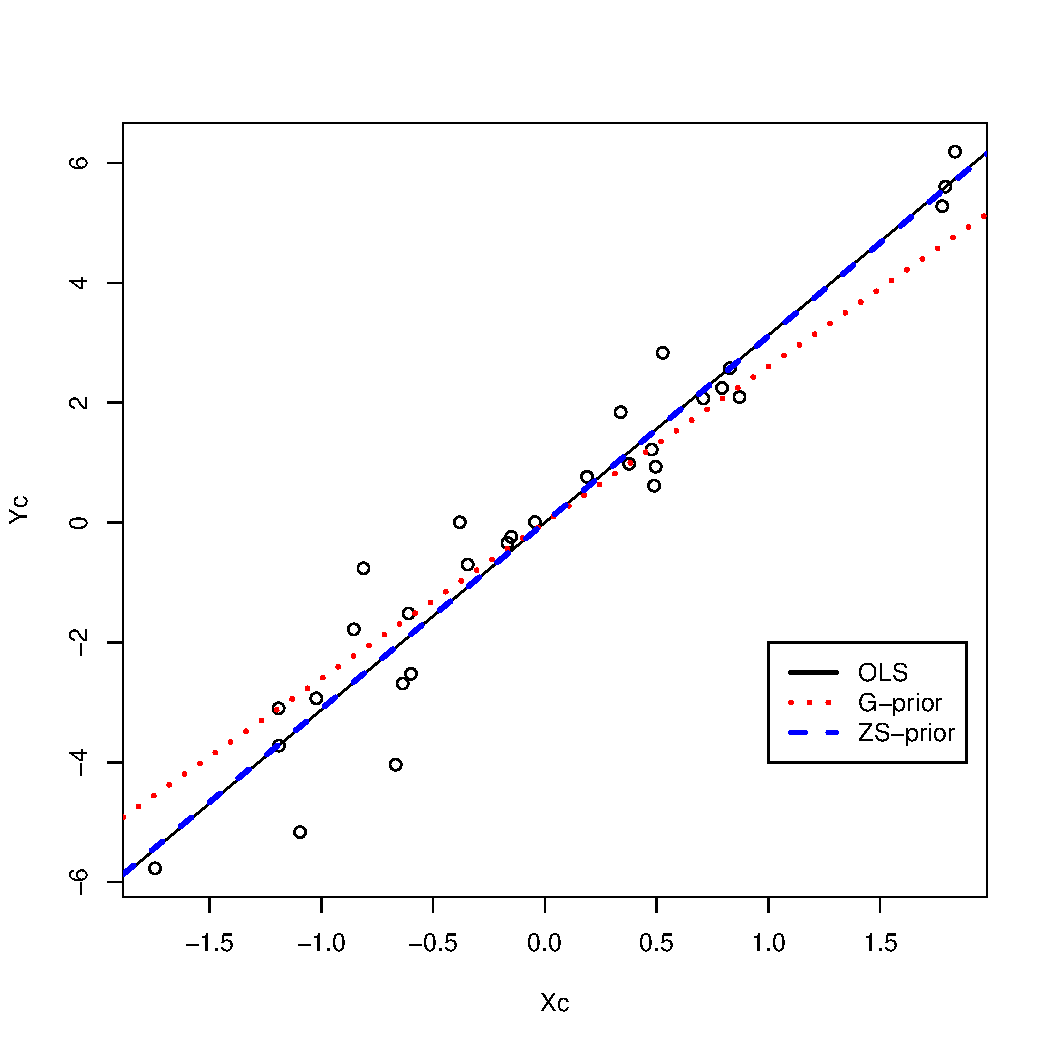
\includegraphics[width=4in,height=3in]{figure/unnamed-chunk-4-1} 

\end{knitrout}

\end{frame}

\begin{frame}[fragile]
\begin{tiny}
\begin{knitrout}
\definecolor{shadecolor}{rgb}{0.969, 0.969, 0.969}\color{fgcolor}\begin{kframe}
\begin{alltt}
\hlstd{ZSout}
\end{alltt}
\begin{verbatim}
## Inference for Bugs model at "/var/folders/n4/nj1122xj6bn5_xgbptv7bml40000gp/T//RtmpfOLtcz/modeld51989ae1ca.txt", fit using jags,
##  3 chains, each with 10000 iterations (first 5000 discarded), n.thin = 5
##  n.sims = 3000 iterations saved
##           mu.vect   sd.vect   2.5%     25%     50%     75%    97.5%  Rhat
## beta        3.112     0.170  2.782   2.997   3.115   3.225    3.445 1.001
## beta0      -0.099     0.152 -0.384  -0.204  -0.099   0.001    0.204 1.002
## g        2263.147 38967.029 48.273 146.129 282.298 697.063 9018.709 1.001
## sigma       0.827     0.114  0.636   0.747   0.816   0.896    1.079 1.001
## deviance   73.347     2.563 70.390  71.458  72.680  74.500   79.882 1.002
##          n.eff
## beta      3000
## beta0     1200
## g         3000
## sigma     3000
## deviance  1600
## 
## For each parameter, n.eff is a crude measure of effective sample size,
## and Rhat is the potential scale reduction factor (at convergence, Rhat=1).
## 
## DIC info (using the rule, pD = var(deviance)/2)
## pD = 3.3 and DIC = 76.6
## DIC is an estimate of expected predictive error (lower deviance is better).
\end{verbatim}
\end{kframe}
\end{knitrout}
\end{tiny}
\end{frame}

\begin{frame}\frametitle{Cauchy Summary}
\begin{itemize}
\item Cauchy rejects prior mean if it is an "outlier"
\item robustness related to "bounded" influence (more later)
\item numerical integration or Monte Carlo sampling (MCMC)
\end{itemize}
\end{frame}
\end{document}


\begin{frame}
  \frametitle{How Good are these Estimators?}
Quadratic loss for estimating  $\b$ using estimator $\a$
$$ L(\b, \a) =  ( \b - \a)^T(\b -\a)$$ \pause

\begin{itemize}
\item Consider our expected loss (before we see the data) of taking an
``action'' $\a$ \pause
\item Under OLS or the  Reference prior the Expected Mean Square Error  \pause
  \begin{eqnarray*}
\E_\Y[( \b - \bhat)^T(\b -\bhat) & = &\sigma^2
  \tr[(\X^T\X)^{-1}] \pause \\
 & = & \sigma^2 \sum_{j=1}^p \lambda_j^{-1}
  \end{eqnarray*}
where $\lambda_j$ are eigenvalues of $\X^T\X$.
\pause
\item If smallest $\lambda_j \to 0$ then MSE  $\to \infty$
\item Note: estimate is unbiased!
\end{itemize}
\end{frame}

\begin{frame}
  \frametitle{Is the $g$-prior better?}

Explore Frequentist properties of using a Bayesian estimator

$$\E_\Y[( \b - \bhat_g)^T(\b -\bhat_g)$$

but now $\bhat_g = g/(1+g) \bhat$
\end{frame}

\begin{frame}\frametitle{Estimator Properties}

  \begin{itemize}
  \item  Bias  \pause
  \item  Variability \pause
  \item MSE = Bias$^2$ + Variance  (multivariate analogs) \pause
\item Problems with OLS \& g-priors with collinearity \pause
\item Solutions: \pause
  \begin{itemize}
  \item removal of terms \pause
   \item other shrinkage estimators
  \end{itemize}

  \end{itemize}
\end{frame}



\end{document}
